\section{Data-Driven Efficiency Modeling}\label{sec:DataDriven}

Fig.~\ref{fig:workflow} illustrates the proposed data-driven workflow, including dataset generation, feature extraction, model training, and design space exploration \cite{Sarada2026}. The workflow is implemented using standard scientific computing and machine learning tools.

\begin{figure*}
    \centering
    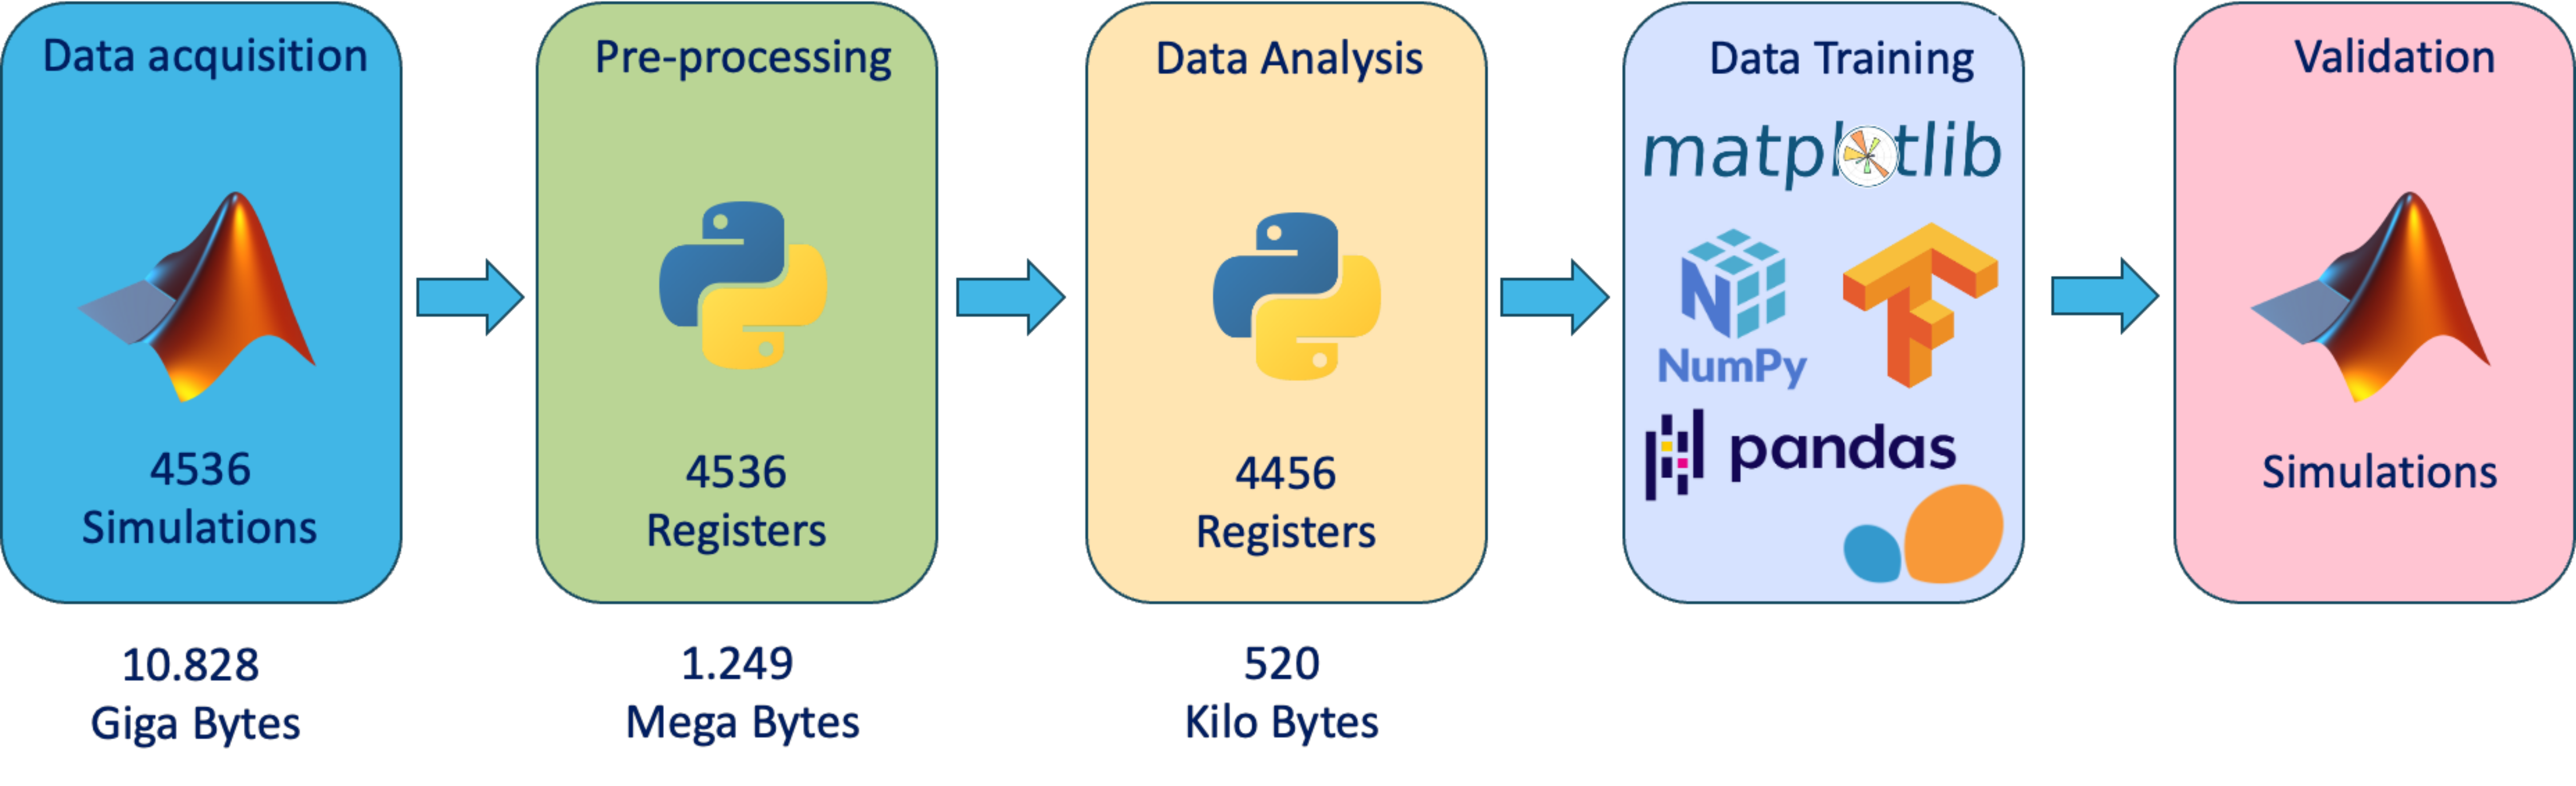
\includegraphics[width=\textwidth]{figures/AI_Steps.png}
    \caption{AI-based efficiency modeling workflow.}
    \label{fig:workflow}
\end{figure*}

The dataset was generated through large-scale time-domain simulations using a detailed LLC converter model implemented in MATLAB/Simulink. The main operating parameters were systematically varied within predefined ranges, including input voltage ($V_{in}$), output voltage ($V_{out}$), output power ($P_{out}$), resonant frequency ($f_r$), and quality factor ($Q$). A similar strategy based on simulation-generated datasets has been adopted in prior work \cite{AvilaSaccol2024}.

For each operating condition, the switching frequency ($f_s$) was swept within a $\pm 1\%$ range around the resonant frequency using seven equally spaced points. This choice focuses the analysis on the region near resonance, where converter efficiency is most sensitive to frequency variations. In total, 4536 scenarios were simulated, generating approximately 10~GB of data.

Each scenario was simulated for 10~ms to ensure steady-state operation. The last 1~ms of data was used for analysis in order to minimize transient effects. Efficiency was computed from the average input and output power over this interval.

To reduce data dimensionality, time-domain signals were summarized using representative scalar features. RMS values were used for currents and AC voltages, while average values were used for DC quantities such as output voltage and power. This representation preserves the steady-state energy behavior of the converter while enabling efficient model training.

After feature extraction, the dataset contained 4536 samples (approximately 1.249 MB). A preprocessing stage was performed to remove outliers, non-physical operating points, and inconsistent data entries. Subsequently, the dataset was divided into training and testing subsets, and all features were normalized to improve numerical stability and model convergence.

Machine learning models have been increasingly applied in power electronics for efficiency prediction and design optimization \cite{zhao2019}. In this work, three regression models were evaluated: Multi-Layer Perceptron (MLP), Random Forest (RF), and K-Nearest Neighbors (KNN), representing different learning approaches. The models estimate converter efficiency as a function of the operating conditions, with input vector $\mathbf{x}$ defined as follows:

\begin{align}
    \mathbf{x} = [V_{in}, V_{out}, P_{out}, f_s, f_r, Z_r, k, Q]
\end{align}

\noindent
where $Z_r = \sqrt{L_r/C_r}$ and $k = L_m / L_r$.

\subsection{Multilayer Perceptron (MLP)}

The MLP was evaluated as a nonlinear regression baseline. The network consists of two hidden layers with 128 and 64 neurons and uses ReLU activation to capture nonlinear relationships, as follows:

\begin{align}
\eta &= f_{\mathrm{MLP}}(\mathbf{x}) \nonumber \\
     &= W_3\,\sigma\!\left(W_2\,\sigma\!\left(W_1 \mathbf{x} + b_1\right) + b_2\right) + b_3
\end{align}

\noindent where $\mathbf{x}$ is the input vector, $W_i$ and $b_i$ are the weights and biases of the layers, respectively, $\sigma$ is the ReLU activation function, and $\eta$ is the predicted efficiency. The model was trained using the Adam optimizer with a learning rate of $10^{-3}$ and mean squared error (MSE) loss, while early stopping was employed to prevent overfitting.

\subsection{Random Forest (RF)}

The Random Forest model was selected as the primary model due to its superior performance. It consists of an ensemble of decision trees trained on bootstrapped data with feature randomness, allowing it to capture nonlinear relationships effectively, it can be written as:

\begin{align}
    \eta &= f_{\mathrm{RF}}(\mathbf{x}) = \frac{1}{N} \sum_{i=1}^{N} T_i(\mathbf{x})
\end{align}

\noindent where $\mathbf{x}$ is the input vector, $T_i(\mathbf{x})$ represents the prediction of the $i$-th decision tree, $N$ is the total number of trees in the ensemble, and $\eta$ is the predicted efficiency obtained from the average of all tree outputs. The model was configured with $N = 300$ trees, a maximum depth of 15, and a minimum of 5 samples per split to improve generalization and reduce overfitting.

\subsection{K Nearest Neighbors (KNN)}

The KNN model was used as a non-parametric baseline. Predictions are obtained by averaging the outputs of the $k$ nearest neighbors in the feature space. It is represented as:

\begin{align}
    \eta &= f_{\mathrm{KNN}}(\mathbf{x}) = \frac{1}{k} \sum_{i \in \mathcal{N}_k(\mathbf{x})} y_i
\end{align}

\noindent where $\mathbf{x}$ is the input vector, $\mathcal{N}_k(\mathbf{x})$ denotes the set of the $k$ nearest neighbors of $\mathbf{x}$, $y_i$ is the target value associated with the $i$-th neighbor, $k = 5$ is the number of neighbors considered, and $\eta$ is the predicted efficiency obtained from the average of the neighboring samples.

\subsection{Model Performance Evaluation}

Model performance was evaluated using $R^2$, RMSE, and prediction error, where $R^2$ measures goodness-of-fit, RMSE provides an absolute error measure, and prediction error (\%) indicates relative accuracy, as summarized in Table~\ref{tab:model_comparison}.

\begin{table}[!htb]
    \centering
    \caption{Performance comparison of machine learning models}
    \label{tab:model_comparison}
    \begin{tabular}{lccc}
        \hline
        Model & $R^2$ & RMSE & Error (\%) \\
        \hline
        MLP & 0.7988 & 0.0872 & 13.01 \\
        RF  & 0.9959 & 0.0125 & 0.78 \\
        KNN & 0.8227 & 0.0819 & 10.08 \\
        \hline
    \end{tabular}
\end{table}

The Random Forest model achieved the best performance, significantly outperforming the other models.

Based on these results, the Random Forest model was used to represent converter efficiency, as follows:

\begin{align}
    \eta &= f_{\mathrm{RF}}(V_{in}, V_{out}, P_{out}, f_s, f_r, Z_r, k, Q)\text{.}
\end{align}

This model enables direct evaluation of the design space without requiring iterative time-domain simulations, where the optimal operating points are identified by formulating the problem as an efficiency maximization under resonant operation and impedance matching constraints. The optimization problem is defined as follows:

\begin{align}
    J &= \eta - \alpha \frac{|f_r - f_s|}{f_s} - \beta \frac{|Z_r - R_{ac}|}{R_{ac}}
\end{align}

\noindent where $J$ is the objective function, $\eta$ is the predicted efficiency, $f_r$ is the resonant frequency, $f_s$ is the switching frequency, $Z_r$ is the resonant tank impedance, $R_{ac}$ is the reflected AC load resistance, and $\alpha = 0.3$ and $\beta = 0.5$ are weighting factors associated with the resonant operation and impedance matching penalties, respectively, balancing efficiency and feasibility.

The optimal point is obtained by solving:

\begin{align}
    \max_{f_s,\,Z_r} \; J \text{.}
\end{align}

This formulation enables efficient exploration of the design space while maintaining physically meaningful operation.

\begin{figure}[htb]
    \centering
    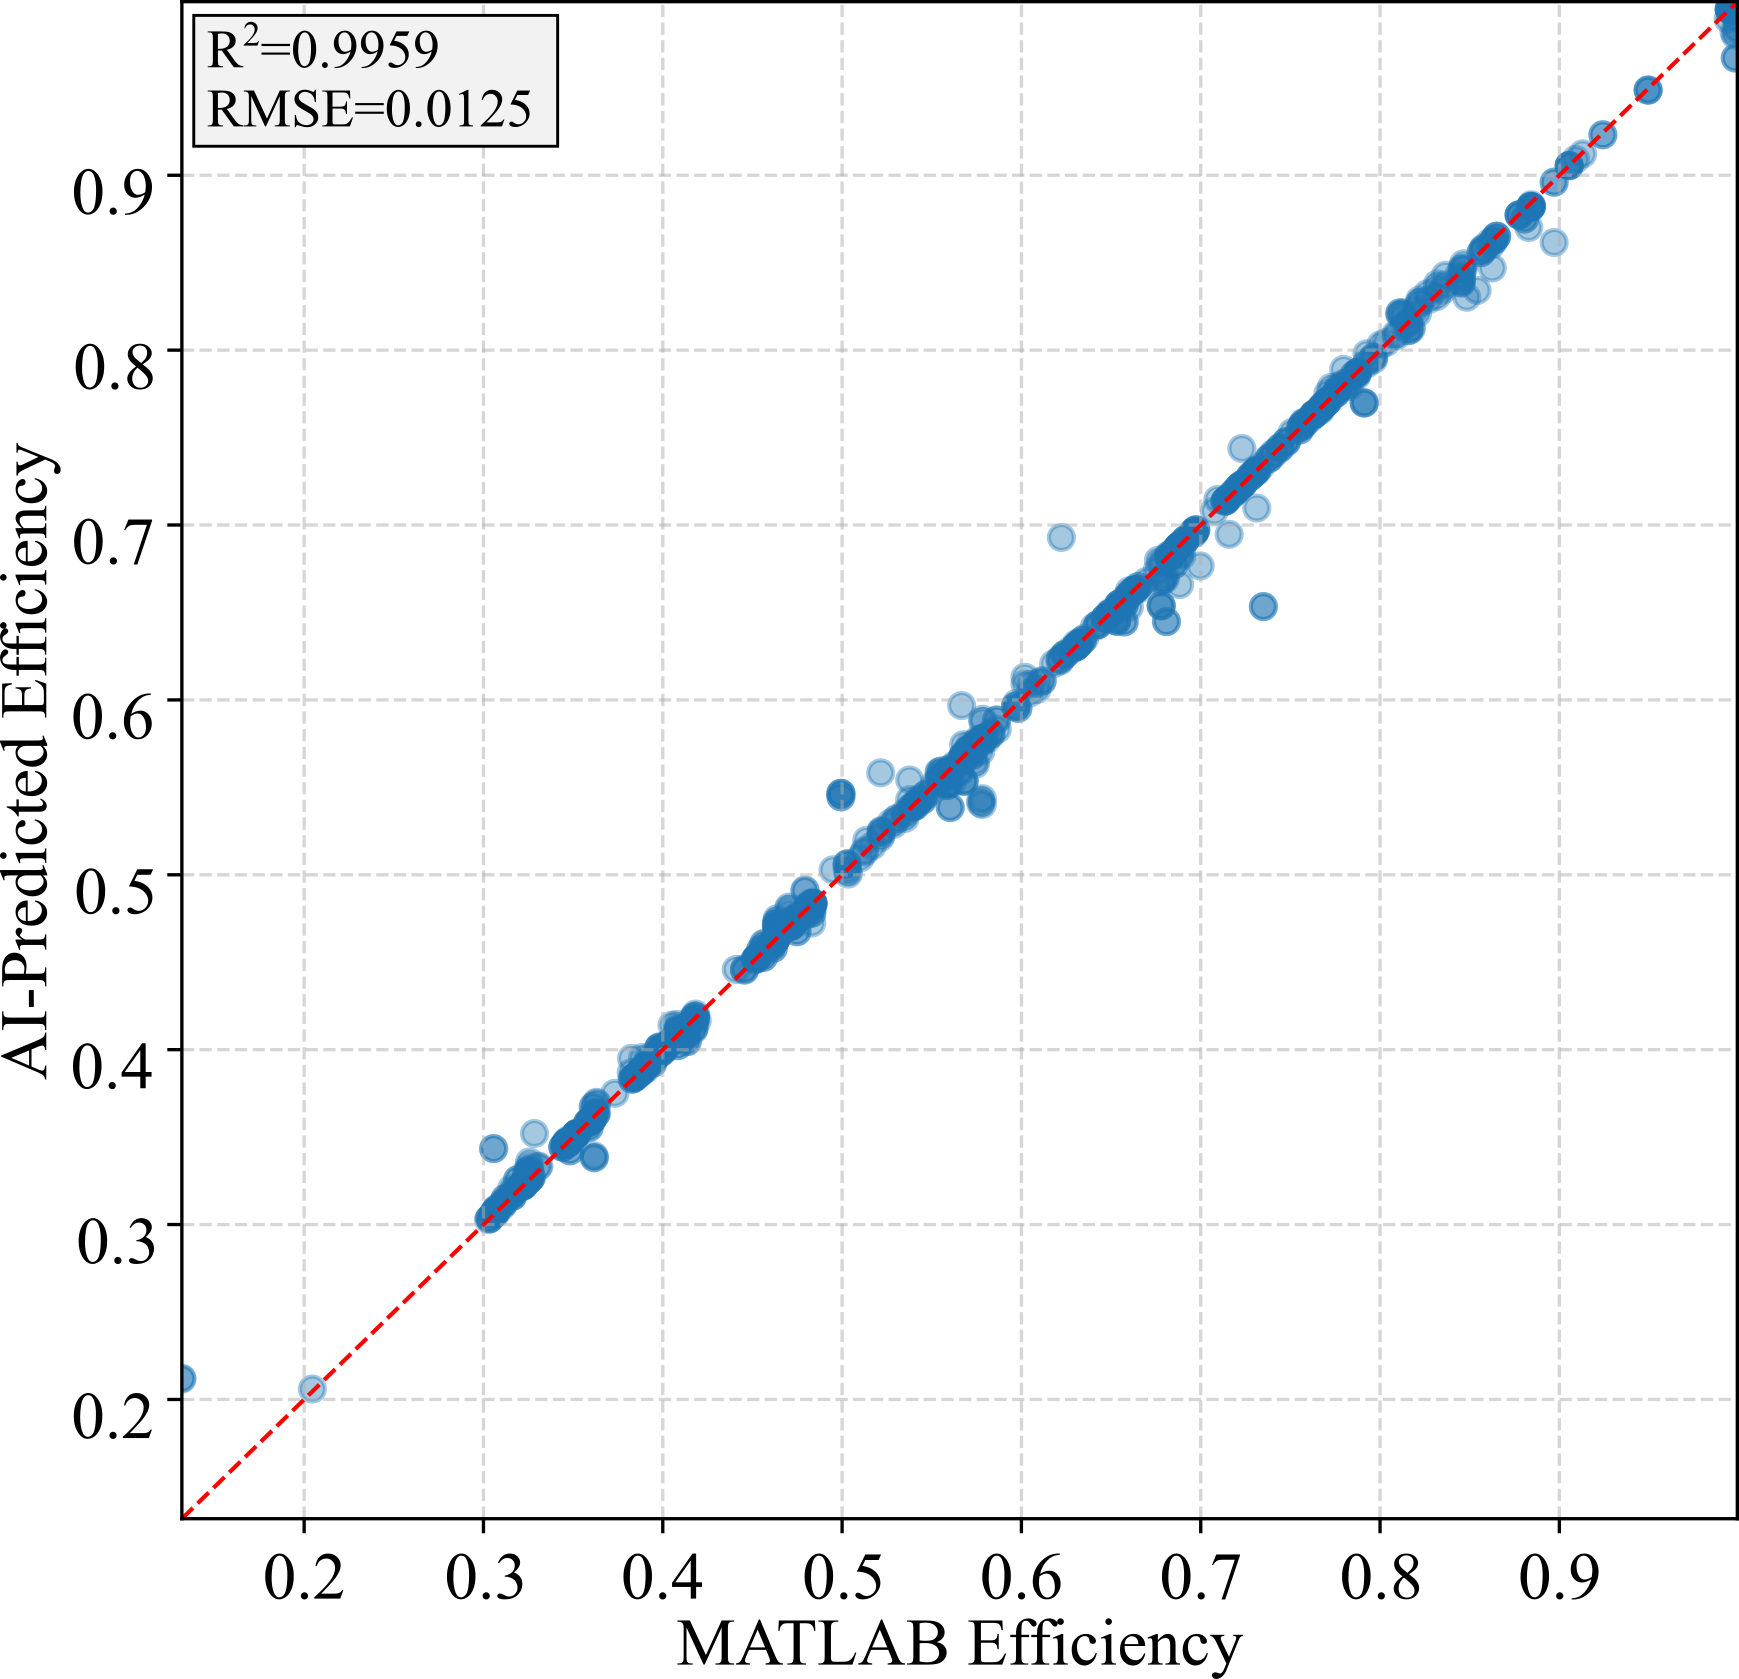
\includegraphics[width=\columnwidth]{figures/RF_Evaluation.png}
    \caption{Predicted versus actual efficiency using the Random Forest model.}
    \label{fig:RF_Evaluation}
\end{figure}

Fig.~\ref{fig:RF_Evaluation} shows strong agreement between the AI-predicted and MATLAB-calculated efficiencies, with the data points closely aligned along the ideal $y = x$ line, confirming the high accuracy and consistency of the model across the operating range.